\documentclass[12pt,titlepage]{article}
%\usepackage{amsmath}
%\usepackage{amsfonts}
%\usepackage{amssymb}
%\usepackage{algorithm}
%\usepackage{algorithmic} 
%
%\usepackage{theorem}
%\usepackage{graphicx}
%
%\usepackage[cp1250]{inputenc}
%\usepackage[T1]{fontenc}
%\usepackage[english]{babel}
%\usepackage[MeX]{polski}
%
%\usepackage{makeidx}
%\usepackage{listings}
%\usepackage{url}
%\usepackage{Here}

\usepackage{graphicx}
\usepackage{graphics}
\usepackage{epsfig}
\usepackage{amsmath}
\usepackage{amssymb}
\usepackage{amsthm}
\usepackage{booktabs}
\usepackage{stmaryrd}
\usepackage{url}
\usepackage{longtable}
\usepackage[figuresright]{rotating}

%\usepackage[MeX]{polski}
\usepackage[cp1250]{inputenc}


\usepackage[T1]{fontenc}
%\usepackage[latin2]{inputenc}
\usepackage[english]{babel}

\usepackage{geometry}
\usepackage{pslatex}
\usepackage{ulem}

\usepackage{lipsum}

\usepackage{listings}
\usepackage{url}
\usepackage{Here}

\usepackage{color}
\definecolor{szary}{gray}{0.6}% jasnoszary

\setlength{\textwidth}{400pt}
\lstset{numbers=left,
			numberstyle=\tiny, 
			basicstyle=\scriptsize\ttfamily, 
			breaklines=true, 
			captionpos=b, 
			tabsize=2}

\usepackage[ruled,vlined,linesnumbered]{algorithm2e}


\selectlanguage{english}

%\vfuzz2pt % Don't report over-full v-boxes if over-edge is small
%\hfuzz2pt % Don't report over-full h-boxes if over-edge is small


\newcommand{\RR}{\mathbb{R}}
\newcommand{\NN}{\mathbb{N}}
\newcommand{\QQ}{\mathbb{Q}}
\newcommand{\ZZ}{\mathbb{Z}}
\newcommand{\TAB}{\hspace{0.50cm}}
\newcommand{\IFF}{\leftrightarrow}
\newcommand{\IMP}{\rightarrow}

\newtheorem{theorem}{Twierdzenie}[section]
\newtheorem{lemma}{Lemat}[section]
\newtheorem{example}{Przyk�ad}[section]
\newtheorem{corollary}{Wniosek}[section]
\newtheorem{definition}{Definicja}[section]

%\newenvironment{proof}{\par\noindent {\bf Dow�d.}}
%{\begin{flushright} \vspace*{-6mm}\mbox{$\Box$} \end{flushright}}
%
%\newenvironment{remark}{\bigskip \par\noindent\begin{small}{\bf Uwaga.}}
%                       {\vspace*{4mm}\end{small}}
%
%\newenvironment{prog}{\par\noindent \sf
%\begin{tabbing}xx\= xx \= xx\= xx\= \kill}
%{\end{tabbing} \rm}


\hyphenation{wszy-stkich ko-lu-mn� ka�-da od-leg-�o��
   dzie-dzi-ny dzie-dzi-na r�w-nych r�w-ny
   pole-ga zmie-nna pa-ra-met-r�w wzo-rem po-cho-dzi
   o-trzy-ma wte-dy wa-run-ko-wych lo-gicz-nie
   skre�-la-na skre�-la-n� ca�-ko-wi-tych wzo-r�w po-rz�-dek po-rz�d-kiem
   przy-k�ad pod-zbio-r�w po-mi�-dzy re-pre-zen-to-wa-ne
   r�w-no-wa�-ne bi-blio-te-kach wy-pro-wa-dza ma-te-ria-��w
   prze-ka-za-nym sko�-czo-nym mo-�esz na-tu-ral-na ci�-gu tab-li-cy
   prze-ka-za-nej}

\makeindex

\begin{document}

\pagestyle{empty}

\begin{titlepage}
\vspace*{\fill}
\begin{center}
\begin{picture}(300,510)
  \put( 10,520){\makebox(0,0)[l]{\large \bf \textsc{Wydzia� Podstawowych Problem�w Techniki}}}
  \put( 10,500){\makebox(0,0)[l]{\large \bf \textsc{Politechniki Wroc�awskiej}}}
  \put( 10,280){\makebox(0,0)[l]{\Huge  \bf \textsc{
  Channels alternative to WiFi in }}}
  \put( 10,260){\makebox(0,0)[l]{\Huge \bf \textsc{
  Authenticated Key Establishment }}}
  \put( 10,240){\makebox(0,0)[l]{\Huge \bf \textsc{
  protocols for mobile devices}}}
  \put(100,200){\makebox(0,0)[l]{\large     \textsc{Pawe� K�dzia}}}

  \put(170, 80){\makebox(0,0)[l]{\large  {In partial fulfillment of the requirements}}}
  \put(170, 60){\makebox(0,0)[l]{\large  {for the degree of Master of Engineering}}}
  \put(170, 40){\makebox(0,0)[l]{\large  { }}}
  \put(170, 20){\makebox(0,0)[l]{\large  {Thesis Supervisor}}}
  \put(170, 0){\makebox(0,0)[l]{\large  {dr in�. �ukasza Krzywieckiego}}}
  \put(100,-80){\makebox(0,0)[bl]{\large \bf \textsc{Wroc�aw 2010}}}
\end{picture}
\end{center}
\vspace*{\fill}
\end{titlepage}

\tableofcontents

\newpage

\pagestyle{headings}

\section*{Introduction}

The goal of the dissertation is to analyse the usability of channels alternative to WiFi in Authenticated Key Establishment (AKE) protocols for mobile devices.
Authentication and communication protocol in audio channel for mobile devices.

Mobile devices to transfer data mainly use Internet. Disadvantage of this method is that network not always is available. In that case one can still transmit data using some another embedded devices like IrDA, Bluetooth or NFC. Unfortunately not every device has these kind of accessories implemented. However, basis of handhelds is to have embedded speaker and microphone. That is why, in this dissertation, to communication between devices were chosen audio channel. Availability audio appliance and a lot of uses of this solution are main advantages. Moreover, the sound waves with appropriate, not to high sound intensity, does not penetrate through the walls. It causing that waves cannot be receive e.g. on the street when some protected data are sending in the house. Furthermore receiver as like sender do not need to known each other (unlike Bluetooth) before starting the communication. Sender just start to transmit data and receiver in the same time listening broadcast.

To authentication and key agreement between mobile devices was choosen Anonymous Mutual Authentication (AMA) protocol, created by L. Hanzlik, K. Klucznik, �. Krzywiecki and M. Kuty�owski. AMA is simmetric, which means  participants execute the same code. One of the advantage is simple to implemented, even on the devices with low power computing. Every key and encryption are sending by audio channel.

Application created on Android system will serve as proof of concept. Application is called AKEBySound. Managed to determine that exist this kind of applications but none of theme are use to authentication and key exchange protocol. To use this app is enough to have mobile phone/smartform with software Android ( version 4.1.2 or higher ), working speaker and microphone, of course.

Dissertation is divided on X parts. The first section focus on analysis of the problem. Explain principal issues used to create the application. Due to the fact protocol is executed by audio channel the first subsection is about sound.  The next one is one of the method to exchange keys on which AMA protocol base - Diffie-Hellman Key exchange.  Tutaj cos o bezpieczenstwie bedzie itp. Dowod poprawnosci protokolu i takie tam.

Next chapter is about System design. In subsections are described assumptions of project and used cases. Then is shown diagram classes 



\section{Analysis of the problem}
\subsection{Sound}
Sound is acoustic wave propagating in different substances such as water, air (so called vibrating wire). These waves are causing auditory sensation and these which in appropriate amplitude and frequency are not detected by human organ of hearing. Sound to spread has to have some medium, that is why not propagate in vacuum. Furthermore sound is longitudinal waves, which means that particles of the medium is in the same direction as the direction of travel of the wave.

\begin{center}
	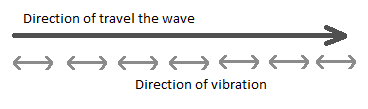
\includegraphics{img/longitudinal_wave}
\end{center}
\subsubsection{Frequency}
Audio frequency is measured in hertz (Hz), where 1 Hz means one cycle per second. Below figures show graphs of audio frequency 1 Hz and 5 Hz.

\begin{center}
	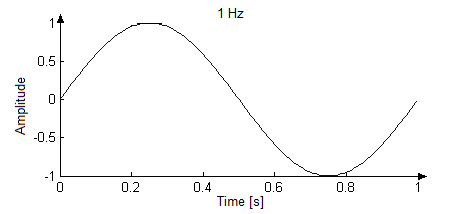
\includegraphics[width=0.45\textwidth]{img/frequency_1Hz}
	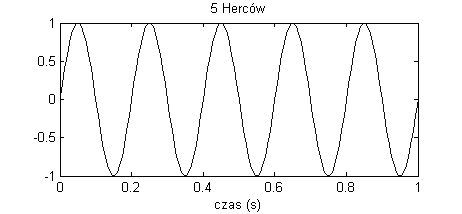
\includegraphics[width=0.45\textwidth]{img/frequency_5Hz}
\end{center}

Exist three division of sound as to frequency:
\begin{itemize}
	\item Infrasound - frequency is lower than 16~Hz.
	\item Hearable sound - frequency is greater than 16~Hz and lower than 20~kHz.
	\item Ultrasound - frequency is greater than 20~kHz.
	\item Hipersound - frequency is greater than 10~GHz.
\end{itemize}

Frequency specify also pitch of sound. A high frequency sound wave corresponds to a high pitch sound and low frequency sound wave corresponds to a low pitch sound.

\subsubsection{Sound intensity}
Loudness of the sound is dependent to his intensity. 

\subsection{Diffie-Hellman Key exchange}
\subsection{Random Oracle Model}

\section{System design}
\subsection{Assumptions}
System should:
\begin{itemize}
	\item Works on every middle class mobile devices with system Android.
	\item Generate keys and encryption during authorization process.
	\item Use sound wave to sending encoded keys and encryptions to another party to establish authorization.
	\item Receiving sound wave and decode received data to keys and encryption from another party to establish authorization.
\end{itemize}
\subsection{Activity diagram}
\subsection{Anonymous Mutual Authentication protocol - Description}

\begin{figure}[here]
	\centering
	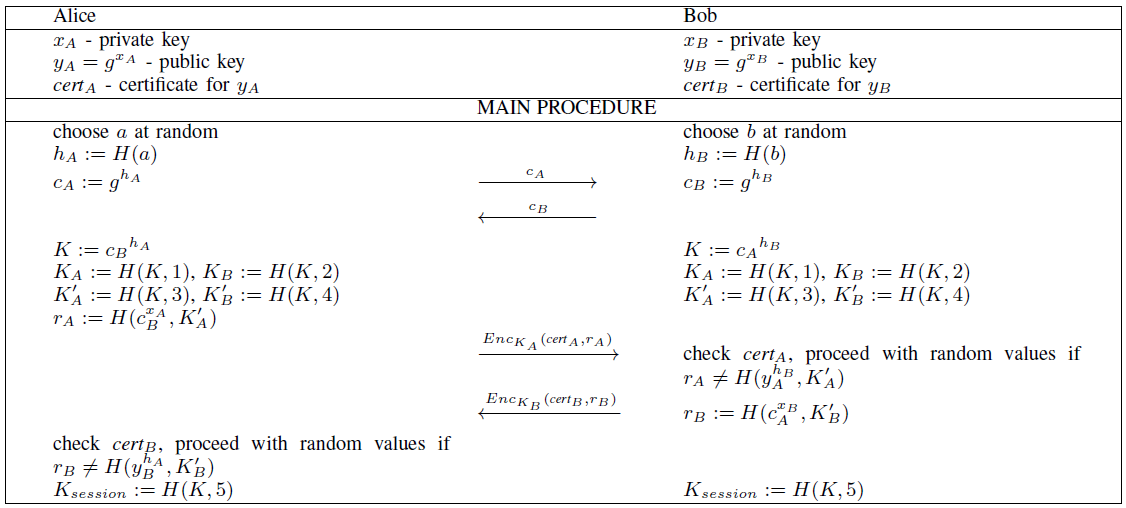
\includegraphics[width=1.2\textwidth]{img/AMA_protocol}
	\caption{Protocol description - Anonymous Mutual Authentication. Figure from source \cite{hammingwindow_img}.}
	\label{fig:F8}
\end{figure}

Scheme of protocol is shown at the Fig. 1. In scheme are use the fallowing notation:
\begin{itemize}
\item \textit{Enc} is a symmetric encryption function. \textit{$Enc_K(M)$} means encryption of $M$ using key $K$. 
\item \textit{H} is a cryptographic hash function. 
\item For confirming public keys are using digital certificates and public key infrastructure (PKI).
\end{itemize}

Protocol is very simple to implement. In the first state, parties (Alice and Bob) generate their private key - $x_A$ (respectively, $x_B$) and public key $y_A = g^{x_A}$ (respectively, $y_A$). Then starts main procedure. Parties generate ephemeral keys. Private is $h_A := H(a)$ (where a is a random number) (respectively $h_B$, b) and public ephemeral key $c_A := g^{h_A}$ (respectively $c_B$). After this parties exchange between themselves public ephemeral key. This is standard Diffie-Hellman key agreement. 

When parties obtain ephemeral public key of another party, start compute master key $K$. Four different one-time keys are establish by hashing $K$ and number parameter - different for each one-time key. 

Authenticated party is raising ephemeral public key $c_B$ (respectively, $c_A$) to power of private key $x_B$ (respectively, $x_A$). On this base authentication. Verifier compute the same value without private key but with the discrete logarithm of $c_A$ (respectively, $c_B$) ($(y_A)^(h_B)$)

\subsubsection{Security model assumption}

\section{Prototype Design}
\subsection{Mobile Devices}

AMA attempts to be simple in implement and does not require high-power computing. So it is ideal to implement it on chip cards. Due to the fact the chip cards are slowly replacing by mobile phones we have decided to implement AMA on this devices. Operating system which we have chosen is Android, because it is one of the most frequently used software on mobile phones. The lowest version, for which program should work without problems is Android 4.1.2. Core of the AMA was implemented in C++. Sound channel and layout was made using Android's libraries. 

\subsection{Operating System}

Operating system which was chosen is Android version 4.1.2 and higher. This is the newest version which was available for device which has been using in tests. Second device to tests has Android 4.2.2. This software has every required libraries whereby is possible to create sound channel between two devices (AudioTrack and AudioRecord). Additionally, Android allows the use of modules written in C++. 

\subsection{Security of Android}

The operating system should ensure that running application cannot interact with another. Each application is run in separate process having  own user ID. This sets up a kernel-level Application Sandbox, where by default application cannot interact with each other and has limited access to OS.

Furthermore, every application has to be signed by developer. Applications without signature will rejected by Google Play or the package installer on Android device. Signed certificate is verified by Package Manager after installation of application.

\subsection{Application architecture}

Application consist of three parts: cryptographic module, sound channel module and graphic interface. Cryptographic module is written in C++ and to use it in Android, was needed to write a wrapper using JNI (Java Native Interface). NDK (Native Development Kit) is a toolset that allows to add native-code languages such as C and C++ to Android's app. User interface consists initial screen where user choose which frequencies have to be use during sending data. In next screen is dynamic graph with recording sound wave and button which start the protocol. To show sound as sinusoid wave we used external library AChartEngine, the rest of interface are created by standard Android's libraries.


Figure 3.

\subsection{Cryptography library}

Exist few of cryptography libraries which are written in Java (e.g. javax.crypto, BouncyCastle), but we wanted to create cryptography module which is independent of the platform. The choice fell on CryptoPP. It is free, open source cryptography library written in C++. The library is objectives and very easy to use. Ensures symmetric and asymmetric cryptography along with signatures and secure hash function. Is used by such companies as Microsoft or Symantec.

\subsection{Activity diagram}

\subsection{NIST recommendation for security parameters}

NIST recommends using 3072 bit length keys to ensure low probability of calculating discrete logarithm. This length is set as default in CryptoPP, however in our prototype we are using 1024 bit. It is caused by duration of sending data by sound. Now, sending 1024 bit length keys take some time and for needs of presentation we decided to stay with this length. For more information please check \cite{NIST}.

\subsection{Shared application model}

\subsection{Java Native Interface - C++ Wrapper}

To be able to use cryptographic part written in C++ in Android, we had to create C++ wrappers using JNI (Java Native Interface) \cite{JNI}. Main class which communicate with C++ code has native methods, for which, after appropriate compilation method, was created MACWrapper.h where definition of methods looks like below.

\begin{lstlisting}
/*
 * Class:     com_example_androidake_MutualAuthenticateChip
 * Method:    prepareMACCPP
 * Signature: (Z)V
 */
JNIEXPORT void JNICALL Java_com_example_androidake_MutualAuthenticateChip_prepareMACCPP
  (JNIEnv *, jobject, jboolean);
\end{lstlisting}

Implementations of methods are in MACWrapper.cpp. There are made conversion from C++ data type to Java data type and vice versa.

\begin{lstlisting}
JNIEXPORT void JNICALL Java_com_example_androidake_MutualAuthenticateChip_prepareMACCPP
(JNIEnv *env, jobject thisObj, jboolean jinit) {
	bool init = jinit;
	if(init == true) {
		mac = new MutualAuthenticationChip(init);
	} else {
		mac_B = new MutualAuthenticationChip(init);
	}
};
\end{lstlisting}

\subsection{Base64}

One of the biggest problem was decided in what representation data should be sending. First choice was standard binary representation with 0 and 1. During creation of sound channel we have found that sending one ephemeral key, which has 1024 bits will take too long. So we decided to reduce sending data using Base64 conversion. Six bits are transform to one of the 64 defined signs. Hence, instead of sending 1024 sings we send just about 172. Data which come from cryptographic module are in Hexadecimal representation. To converse we have used library created by Robert Harder \cite{base_64}. 

\begin{lstlisting}[caption={Example of code converting from Hex String to Base64 String}]
public static String fromHexToBase64(byte[] hex_byte) {
	String hex_str = ConverterJava.ByteToString(hex_byte);
	byte[] decodedHex = null;
	try {
		decodedHex = Hex.decodeHex(hex_str.substring(0,
				hex_str.length() - 1).toCharArray());
	} catch (DecoderException e) {
		e.printStackTrace();
	}
	String encodedHexB64 = Base64.encodeBytes(decodedHex);
	return encodedHexB64;
}
\end{lstlisting}

\subsection{Sound channel}

Sound channel was one of the most difficult part during creation of application. One of the reason was inaccessibility of library whereby we could transform received sound data to cryptographic data. Whole process of analysis received data had to be created from beginning. At beginning we had doubt about sensitivity and precision of speaker and microphone in mobile devices. Especially when we wanted to use ultrasonic waves which could be hard to interpreter. Fortunately, doubts were dispelled after first testing of this channel. Results of working will be describe in Test section. Here we focus on principle of operation.

\subsubsection{Generating sound wave}

Class responsible for generating sound wave get data presented in Base64 (Check section with Base64). Every character A-Z, a-z, 0-9, + and / is mapped to one of the 64 frequencies.

A = 10 kHz,

B = 10,15 kHz,

C = 10,3 kHz,

...

/ = 19,55 kHz


Additional two characters \",\" and \".\" represent begin of data and end of data. Sample rate is 44,1 kHz. Every character is sending during 30 ms, which means that for each pitch is needed 1323 samples. To create sinus wave each sample for $ i \in (0,1322) $ is calculating by formula:
\begin{center}
$\sin($ $Frequency \ast PI \ast 2 \ast i  \over 44 100 $ $)$
\end{center}

These samples are processed by AudioTrack library to sound using PCM encoding. 


\subsubsection{Receiving sound}

Retrieving sound is more complicated than sending. In separate process, using AudioRecord library, in every 15 milliseconds (if sending of one character takes 30 ms), are taken samples and then, as one buffer, are appended to array of buffers. Separate process, in the same time, takes first buffer from array and analyses it. 
 
At this moment, the samples are as short integer values which represent sound in time domain (sinusoid). To check in which frequency was received sound is needed to convert the sampled function from time domain to the frequency domain. We used to this Discrete Transform Fourier. Library which we have chosen to run DFT is \cite{minim_dft}. 

Before change of domain, we need to window samples, using Hanning windowing. Thereby, chart in frequency domain is more readable and is easier to find the place with the highest pitch. Windowed samples are put into DFT method and on the output we have result in frequency domain. The effect on the graph looks like at \ref{fig:F2}.


\begin{figure}[here]
	\centering
	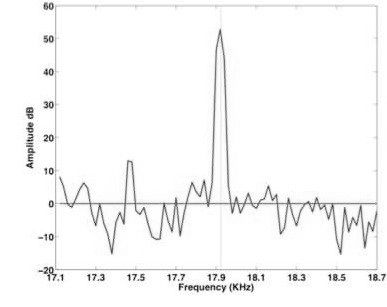
\includegraphics[width=0.45\textwidth]{img/peaks_1}
	\label{fig:F2}
\end{figure}



Now, algorithm tries to find the highest place in the output. The reason of getting data in two times shorter time than sending one character is that, in one buffer can be two frequencies. In the worst case, algorithm can find one frequency in three buffers in a row, even if in first and third buffer was also another frequency, but because of lower sound intensity or less samples representing this frequency, would not be found as a highest pitch. Dividing time of receiving by two ensure that always, at least once, expected frequency will be registered. If he finds pitch with amplitude higher than 50, for frequency lower than 14 kHz, or 10 for higher than 14 kHz (this different follows from the smaller volume for the higher frequency by hardware limitation) is checked whether caught frequency is in our dictionary (with margin of error + - 50 Hz). 

\begin{figure}[here]
	\centering
	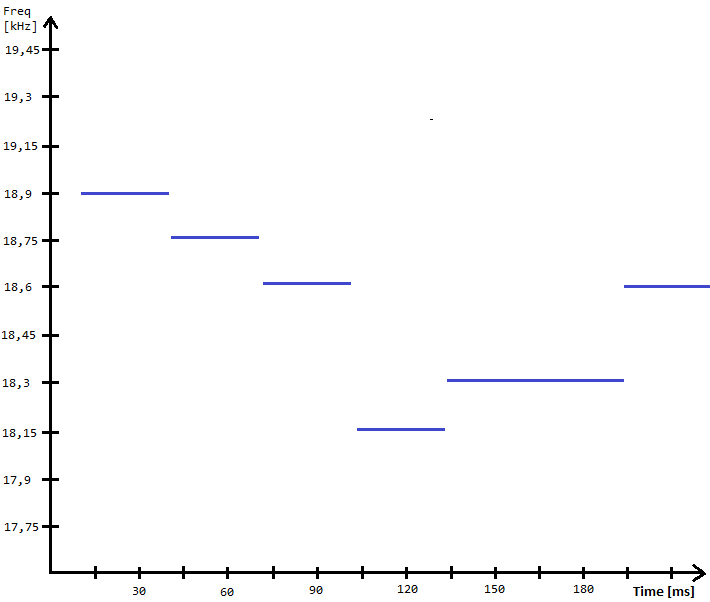
\includegraphics[width=0.70\textwidth]{img/receiving}
	\caption{Figure show received frequencies in time.}
\end{figure}

Caught value is put to the memory and wait for the next result. If current frequency is different than before we change the previous frequency to one of the 64 signs. Otherwise we increment the counter. If counter gain value three (maximal number of occurrences on received character in three further buffers), counter is reset and return adequate character.





\section{Tests}
\section{Installing and implementation}










%%%%%%%%%%%%%%%%%%%%%%%%%%%%%%%%%%%%%%%%%%%%%%%%%%%%%%%%%%%%%%%%%%%%%%%%%%%%%%
%%%%%%%%%%%%%%%%%%%%%%%%%%%%%%% BIBLIOGRAFIA %%%%%%%%%%%%%%%%%%%%%%%%%%%%%%%%%
%%%%%%%%%%%%%%%%%%%%%%%%%%%%%%%%%%%%%%%%%%%%%%%%%%%%%%%%%%%%%%%%%%%%%%%%%%%%%%


\bibliographystyle{plain}

\bibliography{AKESound}


\end{document}
